\documentclass[conference]{IEEEtran}
\usepackage[utf8]{inputenc}
\usepackage[T1]{fontenc}
\usepackage{booktabs}
\usepackage{tabularx}
\usepackage{array}
\usepackage{tikz}
\usetikzlibrary{arrows.meta,positioning,shapes.geometric}
\usepackage{amsmath}
\usepackage{placeins}
\usepackage[hidelinks]{hyperref}

\renewcommand{\IEEEkeywordsname}{Palabras clave}
\renewcommand{\tablename}{Tabla}
\renewcommand{\refname}{Referencias}

\pagestyle{empty}

\begin{document}

% ============================================================
% PORTADA (pagina independiente, una sola columna)
% ============================================================
\begin{titlepage}
\begin{center}
\vspace*{1.5cm}
{\large UNIVERSIDAD T\'ECNICA ESTATAL DE QUEVEDO}\\[0.3cm]
{\normalsize Facultad de Ciencias de la Computaci\'on}\\[0.2cm]
{\normalsize Carrera de Ingenier\'ia de Software}\\[1.2cm]

{\normalsize Asignatura: Aplicaciones Distribuidas (ISR-701)}\\[0.2cm]
{\normalsize Unidad 3 -- Bases de Datos Distribuidas}\\[1.2cm]

{\large\bfseries C\'odigo: TA-IND-02}\\[0.6cm]

{\Large\bfseries An\'alisis de Consistencia y Replicaci\'on en Bases de Datos\\
Distribuidas: el caso del Sistema de Control de\\
Laboratorios Inform\'aticos (SCLI)}\\[1.5cm]

{\normalsize Estudiante: Freddy Farinango}\\[0.2cm]
{\normalsize Equipo PFC: ForaCode}\\[0.2cm]
{\normalsize Proyecto Fin de Curso: Sistema de Control de Laboratorios Inform\'aticos (SCLI)}\\[1.2cm]

{\normalsize Docente: Prof. Guerrero Ulloa G. C.}\\[0.2cm]
{\normalsize Per\'iodo acad\'emico: 2026--2027}\\[0.2cm]
{\normalsize Fecha de entrega: 14/07/2026}\\[1.5cm]

\vfill
{\small Trabajo Aut\'onomo Individual Sumativo -- TA-IND-02}
\end{center}
\end{titlepage}

% ============================================================
% CUERPO ACADEMICO EN DOS COLUMNAS
% ============================================================
\twocolumn

\title{An\'alisis de Consistencia y Replicaci\'on en Bases de Datos Distribuidas:\\
el caso del Sistema de Control de Laboratorios Inform\'aticos (SCLI)}

\author{\IEEEauthorblockN{Freddy Farinango}
\IEEEauthorblockA{Equipo PFC ForaCode\\
Carrera de Ingenier\'ia de Software\\
Universidad T\'ecnica Estatal de Quevedo\\
Aplicaciones Distribuidas (ISR-701)}}

\maketitle

\noindent\textit{\textbf{Resumen}---}El Sistema de Control de Laboratorios Inform\'aticos (SCLI) del equipo ForaCode es una aplicaci\'on Spring Boot que gestiona reservas, asignaciones y asistencia sobre una \'unica instancia de PostgreSQL. Este informe examina, a partir de la revisi\'on directa del c\'odigo fuente y la configuraci\'on del proyecto, el modelo de consistencia realmente implementado. La evidencia indica que el SCLI ofrece \'unicamente consistencia transaccional local bajo el nivel de aislamiento predeterminado de PostgreSQL (\emph{read committed}, al no encontrarse configuraci\'on expl\'icita), sin ninguna estrategia de replicaci\'on demostrable: opera con una sola fuente de datos, transacciones gestionadas por Spring y sin mecanismos de concurrencia optimista o pesimista m\'as all\'a de restricciones \texttt{UNIQUE} puntuales. Se contrastan dos alternativas -- replicaci\'on primario--r\'eplica s\'incrona y as\'incrona -- frente al modelo actual, con criterios de consistencia observada, aislamiento, disponibilidad, latencia, tolerancia a particiones, riesgo de p\'erdida de datos, recuperaci\'on y complejidad operativa. El an\'alisis, enmarcado en CAP y PACELC, concluye que el modelo actual es suficiente para el contexto acad\'emico presente del PFC, pero no constituye una base \'optima para un despliegue con exigencias reales de disponibilidad, y propone una estrategia h\'ibrida de replicaci\'on como mitigaci\'on.

\begin{IEEEkeywords}
consistencia transaccional, replicaci\'on de bases de datos, CAP, PACELC, PostgreSQL, Spring Boot
\end{IEEEkeywords}

% ============================================================
\section{Introducci\'on}

El SCLI es la aplicaci\'on desarrollada por el equipo ForaCode para automatizar la reserva, asignaci\'on y monitoreo de laboratorios inform\'aticos en la UTEQ, junto con el registro de asistencia de estudiantes y docentes. Al tratarse de un sistema donde m\'ultiples usuarios compiten por el mismo recurso f\'isico -- un laboratorio en un horario determinado --, las garant\'ias que ofrece la capa de datos frente a operaciones concurrentes son un aspecto central de su correcci\'on, no un detalle de implementaci\'on secundario.

En sistemas distribuidos, ninguna base de datos replicada ofrece simult\'aneamente consistencia fuerte, disponibilidad total y tolerancia a particiones de red \cite{gilbert2002}. Cuando adem\'as se replica el estado entre nodos, aparece un segundo compromiso, formalizado por PACELC, entre la consistencia y la latencia incluso en ausencia de fallos \cite{abadi2012}. Estas dos tensiones no son abstracciones te\'oricas ajenas al SCLI: determinan qu\'e ocurrir\'ia si dos docentes intentan reservar el mismo laboratorio en el mismo instante bajo una arquitectura replicada, y qu\'e sucede hoy con la disponibilidad del sistema si el \'unico servidor de base de datos deja de responder.

El objetivo de este informe es identificar, con evidencia extra\'ida directamente del c\'odigo fuente y de los archivos de configuraci\'on del SCLI, el modelo de consistencia y la estrategia de replicaci\'on efectivamente implementados, evaluarlos frente al dominio del sistema y contrastarlos con al menos dos alternativas t\'ecnicas. La pregunta que gu\'ia el an\'alisis es: \emph{¿es el modelo de consistencia elegido el \'optimo para el dominio del sistema?} El documento se organiza en un marco te\'orico sobre modelos de consistencia y replicaci\'on, un an\'alisis del modelo real del SCLI, una evaluaci\'on de alternativas, una discusi\'on cr\'itica que responde a la pregunta orientadora, y las conclusiones correspondientes.

% ============================================================
\section{Marco te\'orico}

\subsection{Modelos de consistencia}

La consistencia en sistemas distribuidos no es una propiedad binaria, sino un espectro de garant\'ias ordenadas por su fuerza sem\'antica \cite{viotti2016}. En el extremo m\'as fuerte, la \emph{linealizabilidad} exige que toda operaci\'on parezca ejecutarse de forma instant\'anea en un punto entre su invocaci\'on y su respuesta, de modo que cualquier lector observe siempre el \'ultimo valor escrito por cualquier nodo del sistema. La \emph{consistencia secuencial} relaja esta exigencia temporal pero preserva un orden global \'unico de operaciones compartido por todos los procesos. La \emph{consistencia causal} exige preservar \'unicamente el orden entre operaciones causalmente relacionadas, permitiendo que operaciones concurrentes se observen en \'ordenes distintos en distintas r\'eplicas. La garant\'ia de \emph{lectura de los propios cambios} asegura que un proceso jam\'as deje de ver sus propias escrituras previas, aun cuando no se garantice nada sobre las escrituras de terceros. Finalmente, la \emph{consistencia eventual} solo garantiza que, en ausencia de nuevas escrituras, todas las r\'eplicas converger\'an eventualmente al mismo estado, sin acotar cu\'anto tiempo tomar\'a esa convergencia.

Es importante no confundir este espectro, que describe garant\'ias \emph{entre r\'eplicas}, con las propiedades ACID y los niveles de aislamiento de un motor transaccional que opera sobre una \'unica instancia. La linealizabilidad es una garant\'ia sobre el comportamiento observable de operaciones concurrentes, seg\'un la cual cada operaci\'on parece ejecutarse de manera instant\'anea en un punto comprendido entre su invocaci\'on y su respuesta; en sistemas replicados, preservarla exige coordinaci\'on entre nodos para mantener un orden compatible con el tiempo real. El aislamiento \emph{read committed}, por ejemplo, impide que una transacci\'on lea datos no confirmados por otra, pero no garantiza que distintas transacciones observen un \'unico estado global inmutable ni elimina anomal\'ias como lecturas no repetibles; \emph{serializable} s\'i ofrece esa garant\'ia dentro de un solo nodo, pero ninguno de los dos niveles equivale por s\'i mismo a linealizabilidad. Cuanto m\'as fuerte es el modelo de consistencia distribuida, mayor es la coordinaci\'on necesaria entre nodos antes de confirmar una operaci\'on, lo que incrementa la latencia y reduce la disponibilidad bajo fallos; cuanto m\'as d\'ebil es el modelo, menor es la coordinaci\'on requerida, a costa de exponer al cliente lecturas potencialmente obsoletas.

\subsection{CAP y PACELC}

El teorema CAP demuestra que, ante una partici\'on de red, un sistema distribuido \emph{replicado} no puede garantizar simult\'aneamente consistencia y disponibilidad; debe sacrificar una de las dos mientras la partici\'on persiste \cite{gilbert2002}. Una lectura frecuente pero imprecisa reduce CAP a ``elegir dos de tres propiedades en todo momento''; en realidad, la tolerancia a particiones no es opcional en un sistema verdaderamente distribuido con m\'as de un nodo, por lo que la elecci\'on real ocurre \'unicamente entre C y A, y \'unicamente mientras dura la partici\'on. Cuando solo existe un nodo de datos, no hay una segunda r\'eplica con la cual particionarse, y CAP simplemente no se aplica como clasificaci\'on binaria; el problema relevante en ese caso es otro, y se retoma en la Secci\'on III.

PACELC extiende esta idea al caso, mucho m\'as frecuente en la operaci\'on cotidiana, en que no existe partici\'on: incluso sin fallos de red, un sistema replicado debe elegir entre menor latencia y mayor consistencia, porque coordinar r\'eplicas para garantizar linealizabilidad exige intercambios de mensajes adicionales \cite{abadi2012}. Sistemas de referencia industrial ilustran ambos extremos: Dynamo prioriza la disponibilidad mediante replicaci\'on sin l\'ider y consistencia eventual \cite{decandia2007}, mientras que Spanner ofrece consistencia externa apoy\'andose en sincronizaci\'on temporal de alta precisi\'on entre centros de datos \cite{corbett2013}.

\subsection{Estrategias de replicaci\'on}

La replicaci\'on l\'ider--seguidor (primario--r\'eplica) designa un \'unico nodo que acepta escrituras y uno o m\'as nodos que reciben los cambios de forma s\'incrona o as\'incrona. En el modo s\'incrono, el l\'ider espera la confirmaci\'on de al menos una r\'eplica antes de reconocer la escritura al cliente, lo que evita la p\'erdida de datos ante la ca\'ida del l\'ider a costa de mayor latencia y del riesgo de bloquear escrituras si la r\'eplica no responde. En el modo as\'incrono, el l\'ider confirma la escritura sin esperar a la r\'eplica, reduciendo la latencia percibida pero exponiendo una ventana de posible p\'erdida de transacciones recientes y de lecturas obsoletas (\emph{staleness}, entendida aqu\'i como el retraso entre el momento en que un dato se escribe en el l\'ider y el momento en que se refleja en una r\'eplica) si el l\'ider falla antes de propagar el cambio. Trabajos recientes muestran que sostener consistencia fuerte entre r\'eplicas geogr\'aficamente distribuidas tiene un costo de coordinaci\'on medible y no trivial, que debe compararse expl\'icitamente contra los requisitos reales de la aplicaci\'on antes de adoptarse \cite{du2023}.

La replicaci\'on multi-l\'ider permite que varios nodos acepten escrituras simult\'aneamente, lo que exige resoluci\'on de conflictos cuando dos l\'ideres modifican el mismo dato de forma concurrente. La replicaci\'on sin l\'ider, empleada por sistemas como Dynamo, distribuye lecturas y escrituras entre un conjunto de r\'eplicas y utiliza \emph{quorums} de lectura y escritura para acotar las garant\'ias de consistencia observadas \cite{decandia2007}. Las arquitecturas l\'ider--seguidor, multi-l\'ider y sin l\'ider presentan diferentes compromisos de coordinaci\'on, disponibilidad y resoluci\'on de conflictos \cite{vansteen2017}. La elecci\'on entre estas estrategias contin\'ua siendo un \'area activa de investigaci\'on aplicada, particularmente cuando las transacciones deben mantenerse eficientes sin renunciar a garant\'ias de aislamiento en escenarios multi-regi\'on \cite{nguyen2023}.

\subsection{Consistencia de datos en arquitecturas orientadas a servicios}

La adopci\'on de arquitecturas donde cada servicio administra su propia base de datos traslada buena parte de la responsabilidad de mantener la consistencia desde el motor de base de datos hacia la capa de aplicaci\'on. Un relevamiento reciente de pr\'acticas industriales documenta que los equipos de desarrollo enfrentan de forma recurrente problemas de integridad referencial entre servicios, ausencia de soporte transaccional nativo entre bases de datos independientes y falta de herramientas maduras para depurar fallos de consistencia entre servicios \cite{laigner2021}. Este hallazgo es relevante para el SCLI porque, aunque el sistema no adopta actualmente una descomposici\'on en microservicios, cualquier evoluci\'on futura hacia esa arquitectura heredar\'ia estas mismas tensiones. Un modelo m\'as amplio de los sistemas de datos distribuidos permite adem\'as situar al SCLI dentro de un panorama m\'as general de estrategias de sincronizaci\'on, sean estas basadas en transacciones distribuidas, en propagaci\'on de eventos o en replicaci\'on directa del motor de base de datos \cite{margara2023}.

% ============================================================
\section{An\'alisis del modelo de consistencia y replicaci\'on del SCLI}

\subsection{Arquitectura real identificada}

La revisi\'on del proyecto entregado (\texttt{pom.xml}, directorio \texttt{src/main/java/com/uteq/SCLI}) confirma que el SCLI es una \textbf{aplicaci\'on monol\'itica \'unica} construida con Spring Boot 3.5.4, con un solo m\'odulo Maven (\texttt{groupId com.uteq}, \texttt{artifactId SCLI}) y sin subm\'odulos ni descriptores de microservicios. No se encontr\'o ning\'un \texttt{Dockerfile} ni \texttt{docker-compose.yml} en el proyecto entregado, por lo que no puede afirmarse la existencia de una topolog\'ia de despliegue de m\'ultiples nodos o contenedores; tampoco se dispone de scripts DDL, migraciones versionadas ni archivos de configuraci\'on del servidor PostgreSQL (\texttt{postgresql.conf}, \texttt{pg\_hba.conf}), por lo que cualquier afirmaci\'on sobre el motor de base de datos se limita a lo observable desde la aplicaci\'on.

El archivo \texttt{application.properties} define la propiedad \texttt{spring.datasource.url} con el valor \texttt{jdbc:postgresql://\allowbreak localhost:5432/\allowbreak BD\_Laboratorio1}, con credenciales tomadas de variables de entorno (\texttt{DB\_USER}, \texttt{DB\_PASS}, valores omitidos por seguridad). No existen en el proyecto clases de configuraci\'on de m\'ultiples \texttt{DataSource}, ni perfiles que apunten a hosts distintos: los perfiles \texttt{application-dev.properties} y \texttt{application-prod.properties} \'unicamente ajustan \texttt{spring.jpa.hibernate.ddl-auto} y el cach\'e de Thymeleaf, sin introducir un segundo nodo de base de datos. En consecuencia, el SCLI mantiene una \textbf{\'unica fuente de datos}: una sola instancia de PostgreSQL, sin r\'eplicas de lectura ni nodos de respaldo demostrables en los archivos revisados.

Como se observa en la Fig.~\ref{fig:topologia-actual}, el SCLI depende de una \'unica instancia PostgreSQL y no presenta una r\'eplica demostrable en los archivos revisados.

\begin{figure}[!t]
\centering
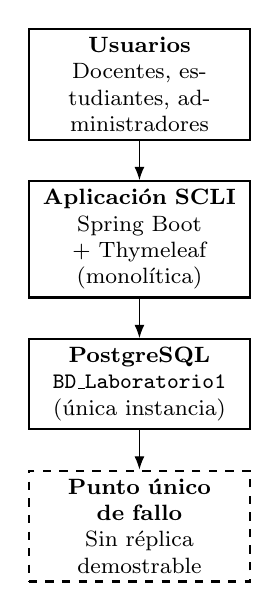
\begin{tikzpicture}[
  font=\footnotesize,
  node distance=0.5cm,
  box/.style={draw, rectangle, text width=2.6cm, minimum height=0.8cm, align=center, thick, inner sep=3pt},
  spofbox/.style={draw, dashed, rectangle, text width=2.6cm, minimum height=0.8cm, align=center, thick, inner sep=3pt}
]
\node[box] (users) {\textbf{Usuarios}\\Docentes, estudiantes, administradores};
\node[box, below=of users] (app) {\textbf{Aplicaci\'on SCLI}\\Spring Boot + Thymeleaf\\(monol\'itica)};
\node[box, below=of app] (dbnode) {\textbf{PostgreSQL}\\\texttt{BD\_Laboratorio1}\\(\'unica instancia)};
\node[spofbox, below=of dbnode] (spof) {\textbf{Punto \'unico de fallo}\\Sin r\'eplica demostrable};

\draw[-{Latex}] (users) -- (app);
\draw[-{Latex}] (app) -- (dbnode);
\draw[-{Latex}] (dbnode) -- (spof);
\end{tikzpicture}
\caption{Topolog\'ia actual del SCLI: aplicaci\'on monol\'itica conectada a una \'unica instancia PostgreSQL, sin r\'eplicas demostrables.}
\label{fig:topologia-actual}
\end{figure}

\subsection{Transacciones y mecanismos de concurrencia}

Se identificaron 20 archivos con anotaciones \texttt{@Transactional}, distribuidas entre repositorios (por ejemplo \texttt{AdminUsuarioRepository}, \texttt{PersonaRepository}), servicios (\texttt{AuthService}, \texttt{SolicitudReservaService}, \texttt{LaboratorioService}, entre otros) y el controlador \texttt{HorarioApiController}. Estas anotaciones delimitan transacciones ACID locales a la instancia \'unica de PostgreSQL, gestionadas por el motor transaccional de Spring; no implican, por s\'i mismas, ninguna forma de replicaci\'on ni de consistencia distribuida. No se encontr\'o ninguna configuraci\'on expl\'icita de nivel de aislamiento (no hay ocurrencias de \texttt{isolation} en las anotaciones revisadas), por lo que las transacciones utilizan previsiblemente el nivel predeterminado de PostgreSQL, \emph{read committed}. Este nivel impide que una transacci\'on lea datos no confirmados por otra, pero no equivale a linealizabilidad ni a consistencia fuerte distribuida, no garantiza que toda transacci\'on observe un \'unico estado inmutable a lo largo de su ejecuci\'on, y no elimina anomal\'ias de concurrencia como las lecturas no repetibles.

Respecto a mecanismos de control de concurrencia adicionales, no se hall\'o ninguna anotaci\'on \texttt{@Version} (bloqueo optimista de JPA), ninguna consulta \texttt{SELECT ... FOR UPDATE}, ninguna palabra clave \texttt{synchronized} ni uso de \texttt{LockModeType} en el c\'odigo fuente revisado. Las \'unicas restricciones de integridad relevantes son \texttt{UNIQUE} a nivel de columna o de tabla: en \texttt{Materia} (\texttt{cod\_materia}), \texttt{Rol} (\texttt{nombre\_rol}), \texttt{Usuario} (\texttt{nombre\_usuario}, y una relaci\'on \texttt{OneToOne} \'unica con \texttt{Persona}), \texttt{Persona} (columna \'unica declarada sin nombre expl\'icito en la anotaci\'on) y \texttt{Equipo} (\texttt{codigo\_equipo}). En las entidades JPA y archivos revisados no se encontr\'o evidencia de una restricci\'on \texttt{UNIQUE} compuesta sobre laboratorio, fecha y franja horaria. Sin embargo, al no disponer del DDL completo, de migraciones versionadas ni de la configuraci\'on real del servidor PostgreSQL, no puede descartarse que exista una restricci\'on, disparador (\emph{trigger}) o funci\'on implementada directamente en la base de datos y ausente en el c\'odigo de aplicaci\'on. Las entidades de dominio m\'as sensibles a este riesgo -- \texttt{AsignacionLaboratorio}, \texttt{SolicitudAsignacion} y \texttt{ReservaEspecial} -- no declaran, en el c\'odigo Java revisado, ninguna restricci\'on \texttt{UNIQUE} compuesta ni mecanismo de bloqueo; con la evidencia disponible, la prevenci\'on de condiciones de carrera en la asignaci\'on de laboratorios parece depender de la l\'ogica de validaci\'on en la capa de servicio, sin que pueda confirmarse ni descartarse una salvaguarda adicional a nivel de motor.

Es relevante notar tambi\'en el uso de \texttt{set\_config} con \'ambito de transacci\'on (\texttt{PgAppContextFilter}, \texttt{DbRoleResetFilter}) para propagar el identificador del docente autenticado como variable de sesi\'on de PostgreSQL, empleada presumiblemente por pol\'iticas de seguridad a nivel de fila. Este mecanismo es inherentemente local a la conexi\'on y a la transacci\'on activa: en una arquitectura con r\'eplicas, este contexto de sesi\'on tendr\'ia que reestablecerse en cualquier nodo que atienda una consulta bajo esas pol\'iticas, lo cual es una consideraci\'on adicional para cualquier estrategia de replicaci\'on futura.

\subsection{Criticidad de los datos por m\'odulo}

No todas las operaciones del SCLI exigen el mismo nivel de exigencia sobre la actualidad del dato le\'ido. Las reservas, asignaciones de laboratorio, control de horarios, registro de asistencia, gesti\'on de usuarios y de roles/permisos requieren controles de concurrencia que eviten dobles asignaciones o actualizaciones incompatibles. La existencia de una \'unica fuente elimina la divergencia entre r\'eplicas, pero el aislamiento \emph{read committed} no evita por s\'i solo todas las condiciones de carrera: cada sentencia observa una instant\'anea de los datos confirmados al inicio de su ejecuci\'on, sin garantizar resultados serializables ante operaciones concurrentes sobre el mismo recurso. En contraste, los reportes agregados, los paneles informativos y las consultas anal\'iticas no cr\'iticas (evidenciados en el paquete \texttt{controller.ReporteControllerFreddy} y las vistas de \texttt{dashboard/admin/reportes}) podr\'ian tolerar datos ligeramente atrasados sin afectar la correcci\'on funcional del sistema, siempre que el retraso se mantenga acotado y se comunique al usuario.

\subsection{Lectura CAP/PACELC del modelo actual}

Una arquitectura de nodo \'unico no implementa, en sentido estricto, tolerancia a particiones: no existe un segundo nodo con el cual particionarse. Por ello no es correcto calificar al SCLI como ``CP'' o ``AP''; ambas etiquetas presuponen una topolog\'ia replicada, y CAP se vuelve decisivo \'unicamente cuando se introducen r\'eplicas y aparece la posibilidad de una partici\'on entre nodos de datos. Lo que s\'i puede afirmarse es que la ca\'ida de la \'unica instancia de PostgreSQL produce la p\'erdida total de disponibilidad del sistema, sin que exista ning\'un nodo de respaldo que asuma el servicio. Esto constituye un \textbf{punto \'unico de fallo} (\emph{single point of failure}) tanto a nivel de datos como, potencialmente, a nivel de aplicaci\'on si esta se despliega en una sola instancia. Bajo PACELC, al no existir r\'eplicas, el sistema no enfrenta el compromiso entre latencia y consistencia que s\'i aparecer\'ia al introducir replicaci\'on: la baja complejidad operativa actual y la ausencia de coordinaci\'on entre nodos tienen como contrapartida que cualquier falla de la \'unica instancia detiene por completo el servicio.

\subsection{Limitaciones de la evidencia disponible}

El ZIP entregado no incluye scripts de creaci\'on del esquema (DDL) ni migraciones versionadas; la estructura de tablas se infiere \'unicamente de las anotaciones JPA de las entidades. Tampoco se incluyen archivos de configuraci\'on de PostgreSQL ni evidencia de un entorno de despliegue (contenedores, orquestaci\'on) m\'as all\'a del c\'odigo de la aplicaci\'on. El an\'alisis presentado se limita, por tanto, a lo demostrable a partir del c\'odigo fuente, las propiedades de Spring y los archivos de configuraci\'on incluidos en el proyecto; donde la evidencia es incompleta, este informe lo indica expl\'icitamente en lugar de asumir una ausencia absoluta.

% ============================================================
\section{Evaluaci\'on de alternativas}

\subsection{Modelo actual: instancia \'unica}

Como se describi\'o en la Secci\'on III, todas las lecturas del SCLI se dirigen a una \'unica fuente de datos, por lo que no existe divergencia entre r\'eplicas. El aislamiento \emph{read committed} evita la lectura de datos no confirmados, pero no garantiza serializaci\'on de todas las operaciones concurrentes ni equivale a linealizabilidad. Esta \'ultima constituye una garant\'ia distinta sobre el orden observable de las operaciones y, en una arquitectura replicada, requiere coordinaci\'on entre nodos. El costo del modelo actual es la ausencia total de tolerancia a fallos del nodo de datos.

\subsection{Alternativa 1: replicaci\'on primario--r\'eplica s\'incrona}

En este modelo, el nodo primario espera la confirmaci\'on de al menos una r\'eplica s\'incrona antes de reconocer la escritura. Para el SCLI, esto preservar\'ia la consistencia transaccional ya existente en las operaciones cr\'iticas (reservas, asignaciones, asistencia, usuarios y permisos) mientras ofrece un nodo adicional con una copia de los datos ante la ca\'ida del primario. La incorporaci\'on de una r\'eplica s\'incrona puede \textbf{reducir}, mas no eliminar por s\'i sola, el punto \'unico de fallo del almacenamiento: para que efectivamente mejore la disponibilidad se requiere adem\'as detecci\'on de fallos, promoci\'on controlada de la r\'eplica a primario (que no ocurre autom\'aticamente salvo que exista una herramienta de orquestaci\'on configurada para ello), redirecci\'on de conexiones de la aplicaci\'on hacia el nuevo primario, monitoreo continuo y procedimientos de \emph{failover} probados peri\'odicamente; de lo contrario pueden persistir puntos \'unicos de fallo adicionales en la aplicaci\'on, la red o el balanceador. El costo es una mayor latencia por confirmaci\'on de escritura y la posibilidad de que las escrituras se detengan o bloqueen si la r\'eplica s\'incrona requerida no responde. Ante una partici\'on de red entre el primario y su r\'eplica s\'incrona, el sistema deber\'ia decidir expl\'icitamente entre rechazar temporalmente las escrituras (preservando consistencia) o degradar a un modo de menor garant\'ia (preservando disponibilidad); para operaciones de reserva y asignaci\'on, rechazar temporalmente la operaci\'on es preferible a permitir una doble asignaci\'on que luego deba revertirse manualmente. Como se\~nalan estudios recientes sobre el costo de la consistencia fuerte en r\'eplicas geo-distribuidas, esta coordinaci\'on adicional no es gratuita y debe dimensionarse contra el volumen real de escrituras concurrentes del sistema \cite{du2023}.

\subsection{Alternativa 2: replicaci\'on primario--r\'eplica as\'incrona}

Aqu\'i el primario confirma la escritura sin esperar a la r\'eplica, reduciendo la latencia de escritura percibida por el usuario. El riesgo es la p\'erdida de transacciones recientes si el primario falla antes de propagar el cambio, y que las lecturas dirigidas a la r\'eplica reflejen un estado ligeramente atrasado. Esta alternativa resulta \'util para descargar del nodo primario las consultas de reportes, paneles informativos y estad\'isticas de uso -- operaciones que, seg\'un el an\'alisis de criticidad de la Secci\'on III, toleran cierto grado de \emph{staleness} -- sin comprometer la consistencia transaccional de las operaciones cr\'iticas, que continuar\'ian at\'endose exclusivamente en el primario. Ninguna de las dos alternativas, por s\'i sola, garantiza alta disponibilidad: ambas requieren monitoreo continuo, procedimientos de recuperaci\'on probados y, en el caso s\'incrono, un mecanismo de \emph{failover} verificado peri\'odicamente.

\subsection{Tabla comparativa}

La Tabla~\ref{tab:comparacion-modelos} presenta los principales compromisos t\'ecnicos entre el modelo actual y las dos alternativas evaluadas. Ninguna celda debe interpretarse como una garant\'ia absoluta: la disponibilidad de la replicaci\'on s\'incrona, por ejemplo, depende de que el mecanismo de \emph{failover} est\'e correctamente configurado y probado, y no es autom\'atica por el solo hecho de introducir una r\'eplica.

\begin{table*}[!t]
\centering
\caption{Comparaci\'on entre el modelo actual del SCLI y dos alternativas de replicaci\'on.}
\label{tab:comparacion-modelos}
\small
\begin{tabularx}{\textwidth}{@{}l X X X@{}}
\toprule
\textbf{Criterio} & \textbf{Modelo actual (instancia \'unica)} & \textbf{R\'eplica s\'incrona} & \textbf{R\'eplica as\'incrona} \\
\midrule
Consistencia observada & Transaccional local bajo \emph{read committed} presumible; sin divergencia entre r\'eplicas porque no existen r\'eplicas & Transaccional local, extendida a la r\'eplica confirmada antes del commit & Transaccional local en el primario; r\'eplica con posible retraso \\
Aislamiento y concurrencia & \emph{Read committed} presumible; sin bloqueo optimista ni pesimista expl\'icito & Igual que el actual en el primario; agrega coordinaci\'on de commit & Igual que el actual en el primario; r\'eplica de solo lectura \\
Disponibilidad & Nula ante ca\'ida del \'unico nodo & Mejorada solo si el \emph{failover} est\'a configurado, monitoreado y probado & Mejorada para lecturas; la escritura sigue dependiendo del primario \\
Latencia de escritura & Baja (sin coordinaci\'on) & Mayor (espera confirmaci\'on de la r\'eplica) & Baja (no espera a la r\'eplica) \\
Tolerancia a particiones & No aplica (nodo \'unico) & Requiere decidir entre rechazar escrituras o degradar el servicio & Favorece disponibilidad; la r\'eplica puede quedar desactualizada \\
Riesgo de p\'erdida de datos & Bajo dentro del nodo \'unico & Bajo (la r\'eplica confirma antes del commit) & Existe una ventana entre el commit y la propagaci\'on \\
Recuperaci\'on ante fallos & Sin nodo de respaldo; requiere restaurar desde copia de seguridad & Failover hacia la r\'eplica, si fue probado y monitoreado previamente & Failover posible, con riesgo de perder transacciones recientes \\
Complejidad operativa & Baja & Alta: monitoreo, promoci\'on de r\'eplica, pruebas peri\'odicas de recuperaci\'on & Media: monitoreo del retraso de replicaci\'on \\
Adecuaci\'on al SCLI & Suficiente para el contexto acad\'emico actual del PFC & Adecuada para reservas, asignaciones y asistencia & Adecuada para reportes e indicadores no cr\'iticos \\
\bottomrule
\end{tabularx}
\end{table*}

\subsection{Recomendaci\'on argumentada}

La arquitectura recomendada se representa en la Fig.~\ref{fig:topologia-propuesta}. Una estrategia h\'ibrida resulta m\'as adecuada que adoptar un \'unico esquema de replicaci\'on para todas las operaciones: r\'eplica s\'incrona para las operaciones cr\'iticas identificadas en la Secci\'on III (reservas, asignaciones, asistencia, usuarios, permisos) y r\'eplica as\'incrona -- o consultas dirigidas a la misma r\'eplica s\'incrona en modo de solo lectura -- para reportes e indicadores no cr\'iticos. Esta propuesta no equivale por s\'i sola a alta disponibilidad: requiere infraestructura adicional para alojar al menos un nodo de r\'eplica, administraci\'on y monitoreo continuo del estado de replicaci\'on, un procedimiento de \emph{failover} documentado y probado peri\'odicamente (no autom\'atico por defecto), restricciones de integridad adicionales a nivel de motor, y pruebas de recuperaci\'on ante fallos que hoy no existen en el proyecto revisado.

\begin{figure*}[!t]
\centering
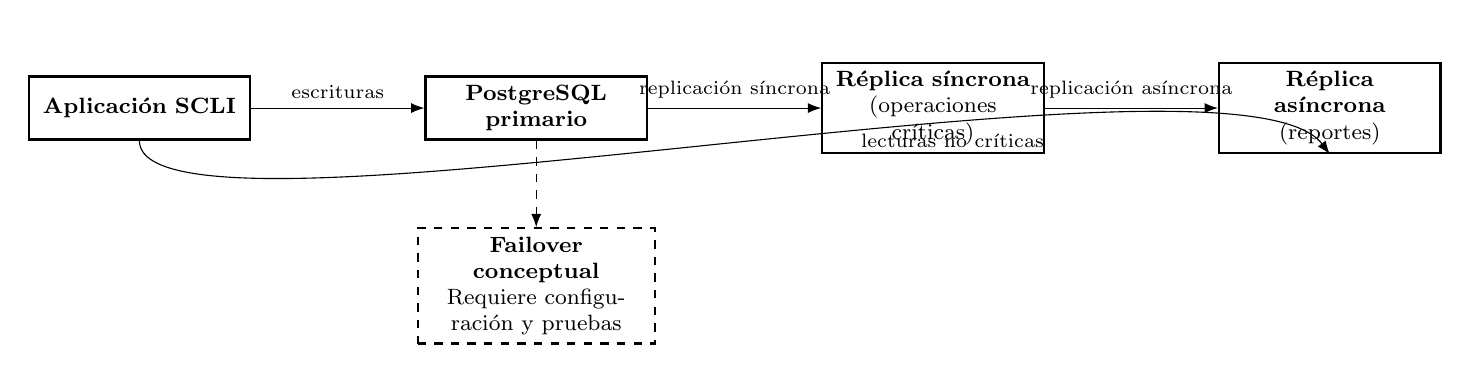
\begin{tikzpicture}[
  font=\footnotesize,
  node distance=1.4cm and 2.2cm,
  box/.style={draw, rectangle, text width=2.6cm, minimum height=0.8cm, align=center, thick, inner sep=3pt},
  spofbox/.style={draw, dashed, rectangle, text width=2.8cm, minimum height=0.8cm, align=center, thick, inner sep=3pt}
]
\node[box] (app) {\textbf{Aplicaci\'on SCLI}};
\node[box, right=of app] (primary) {\textbf{PostgreSQL primario}};
\node[box, right=of primary] (sync) {\textbf{R\'eplica s\'incrona}\\(operaciones cr\'iticas)};
\node[box, right=of sync] (async) {\textbf{R\'eplica as\'incrona}\\(reportes)};
\node[spofbox, below=1.1cm of primary] (failover) {\textbf{Failover conceptual}\\Requiere configuraci\'on y pruebas};

\draw[-{Latex}] (app) -- (primary) node[midway, above, font=\scriptsize] {escrituras};
\draw[-{Latex}] (primary) -- (sync) node[midway, above, font=\scriptsize] {replicaci\'on s\'incrona};
\draw[-{Latex}] (sync) -- (async) node[midway, above, font=\scriptsize] {replicaci\'on as\'incrona};
\draw[-{Latex}] (app.south) .. controls +(0,-1.6) and +(-1.2,1.6) .. (async.south) node[pos=0.65, below, font=\scriptsize] {lecturas no cr\'iticas};
\draw[dashed, -{Latex}] (primary) -- (failover);
\end{tikzpicture}
\caption{Topolog\'ia propuesta para el SCLI: r\'eplica s\'incrona para operaciones cr\'iticas y r\'eplica as\'incrona para consultas no cr\'iticas.}
\label{fig:topologia-propuesta}
\end{figure*}

\FloatBarrier

% ============================================================
\section{Discusi\'on cr\'itica}

¿Es el modelo de consistencia elegido el \'optimo para el dominio del sistema? La respuesta, a partir de la evidencia recogida, es \textbf{matizadamente negativa}: el modelo actual es razonable como soluci\'on transitoria para un proyecto acad\'emico en desarrollo, pero no constituye una base adecuada para un despliegue en producci\'on que deba garantizar continuidad de servicio.

A favor del modelo actual puede reconocerse que ofrece consistencia transaccional local sin ning\'un costo de coordinaci\'on entre nodos: todas las consultas acceden a la misma instancia, por lo que no existe divergencia entre r\'eplicas; no obstante, el comportamiento concurrente continúa condicionado por el aislamiento \emph{read committed} y por los controles de integridad disponibles, y no por una propiedad de consistencia distribuida que el sistema no implementa. Esto simplifica considerablemente el desarrollo y es adecuado mientras el volumen de usuarios concurrentes y la exigencia de disponibilidad continua se mantengan bajos, como corresponde a un sistema en fase de proyecto de curso. Sin embargo, sus limitaciones son sustanciales: el punto \'unico de fallo identificado en la Secci\'on III implica que cualquier interrupci\'on del \'unico servidor de PostgreSQL -- por mantenimiento, saturaci\'on de recursos o fallo de hardware -- deja al sistema completamente inoperativo, sin capacidad de degradar el servicio de forma controlada. Adicionalmente, no se encontr\'o evidencia de restricciones \texttt{UNIQUE} compuestas ni de bloqueos expl\'icitos en las entidades de reserva y asignaci\'on en el c\'odigo Java revisado -- sin que ello permita descartar de forma absoluta una salvaguarda a nivel de motor no visible en los archivos entregados --, lo cual es una condici\'on fr\'agil frente a picos de concurrencia reales, como el inicio de un per\'iodo de matr\'iculas.

Le\'ido bajo CAP, el sistema no ejerce hoy ninguna decisi\'on expl\'icita entre consistencia y disponibilidad porque no hay r\'eplicas con las cuales particionarse; esa decisi\'on queda pospuesta, no resuelta, y se volver\'a decisiva en cuanto se introduzca una segunda instancia de datos. Le\'ido bajo PACELC, el sistema tampoco enfrenta hoy el compromiso entre latencia y consistencia propio de las arquitecturas replicadas, pero a cambio asume el riesgo m\'aximo de disponibilidad. La mitigaci\'on concreta que se propone es la incorporaci\'on de al menos una r\'eplica s\'incrona para las operaciones cr\'iticas, acompa\~nada de restricciones \texttt{UNIQUE} compuestas (laboratorio, fecha, franja horaria) que blinden a nivel de motor de base de datos lo que hoy parece depender \'unicamente de la capa de aplicaci\'on. Para el contexto actual del PFC -- entorno acad\'emico, volumen de usuarios acotado, sin obligaci\'on contractual de disponibilidad continua --, el modelo de instancia \'unica es \emph{suficiente}; para un eventual despliegue institucional real, con exigencias de continuidad de servicio durante per\'iodos acad\'emicos cr\'iticos, no es \'optimo.

% ============================================================
\section{Conclusiones}

La revisi\'on del proyecto permiti\'o verificar que el SCLI implementa consistencia transaccional local sobre una \'unica instancia de PostgreSQL, con aislamiento presumiblemente \emph{read committed} al no encontrarse configuraci\'on expl\'icita, y sin ninguna estrategia de replicaci\'on demostrable en \texttt{application.properties} ni en la ausencia de m\'ultiples \texttt{DataSource}, \texttt{Dockerfile} o \texttt{docker-compose.yml} en el proyecto entregado. El aislamiento \emph{read committed} evita la lectura de datos no confirmados, pero no equivale a linealizabilidad: esta \'ultima es una garant\'ia distinta sobre el orden observable de las operaciones concurrentes que, en una arquitectura replicada, requerir\'ia coordinaci\'on expl\'icita entre nodos.

Frente a la pregunta orientadora, el modelo actual no es el \'optimo para un dominio que involucra reservas concurrentes de recursos f\'isicos limitados y que aspira a una eventual operaci\'on institucional continua: la ausencia de un nodo de respaldo constituye un punto \'unico de fallo, y la ausencia de evidencia de restricciones a nivel de motor para combinaciones laboratorio--horario deja la integridad de las reservas dependiendo, hasta donde permite verificar la evidencia disponible, de la l\'ogica de aplicaci\'on. La alternativa recomendada es una estrategia h\'ibrida de replicaci\'on primario--r\'eplica, s\'incrona para operaciones cr\'iticas y as\'incrona (o de solo lectura sobre la misma r\'eplica) para reportes, que preserva la consistencia donde es indispensable y mejora la disponibilidad general del sistema a un costo de complejidad operativa acotado, siempre que se acompa\~ne de pruebas de \emph{failover} y recuperaci\'on peri\'odicas.

Este estudio se limita a lo verificable en el c\'odigo fuente y la configuraci\'on entregados; no se dispuso de los scripts de esquema de base de datos ni de la configuraci\'on de despliegue real del PFC, por lo que cualquier decisi\'on de arquitectura de replicaci\'on requerir\'ia validarse adicionalmente contra el volumen real de usuarios concurrentes y los requisitos institucionales de continuidad de servicio del equipo ForaCode.

\FloatBarrier

% ============================================================
\section*{Declaraci\'on de uso de inteligencia artificial generativa}

Se utiliz\'o Claude, de Anthropic, como herramienta de apoyo para organizar la estructura del documento, aclarar conceptos t\'ecnicos y revisar la redacci\'on acad\'emica. El an\'alisis del c\'odigo fuente, la interpretaci\'on del modelo de consistencia, la validaci\'on de los hallazgos, la selecci\'on y comprobaci\'on de las referencias, la evaluaci\'on de alternativas y las conclusiones fueron revisadas y validadas por el autor. La herramienta no fue utilizada como fuente bibliogr\'afica.

% ============================================================
\begin{thebibliography}{00}

\bibitem{abadi2012} D. J. Abadi, ``Consistency Tradeoffs in Modern Distributed Database System Design: CAP is Only Part of the Story,'' \emph{Computer}, vol. 45, no. 2, pp. 37--42, 2012. doi: 10.1109/MC.2012.33

\bibitem{corbett2013} J. C. Corbett \emph{et al.}, ``Spanner: Google's Globally Distributed Database,'' \emph{ACM Transactions on Computer Systems}, vol. 31, no. 3, pp. 1--22, 2013, art. no. 8. doi: 10.1145/2491245

\bibitem{decandia2007} G. DeCandia \emph{et al.}, ``Dynamo: Amazon's Highly Available Key-value Store,'' in \emph{Proc. 21st ACM SIGOPS Symposium on Operating Systems Principles (SOSP '07)}, 2007, pp. 205--220. doi: 10.1145/1294261.1294281

\bibitem{gilbert2002} S. Gilbert and N. Lynch, ``Brewer's Conjecture and the Feasibility of Consistent, Available, Partition-Tolerant Web Services,'' \emph{ACM SIGACT News}, vol. 33, no. 2, pp. 51--59, 2002. doi: 10.1145/564585.564601

\bibitem{vansteen2017} M. van Steen and A. S. Tanenbaum, \emph{Distributed Systems}, 3rd ed. distributed-systems.net, 2017. ISBN 978-1543057386.

\bibitem{viotti2016} P. Viotti and M. Vukoli\'c, ``Consistency in Non-Transactional Distributed Storage Systems,'' \emph{ACM Computing Surveys}, vol. 49, no. 1, pp. 1--34, 2016, art. no. 19. doi: 10.1145/2926965

\bibitem{laigner2021} R. Laigner, Y. Zhou, M. A. Vaz Salles, Y. Liu, and M. Kalinowski, ``Data Management in Microservices: State of the Practice, Challenges, and Research Directions,'' \emph{Proceedings of the VLDB Endowment}, vol. 14, no. 13, pp. 3348--3361, 2021. doi: 10.14778/3484224.3484232

\bibitem{nguyen2023} C. D. T. Nguyen, J. K. Miller, and D. J. Abadi, ``Detock: High Performance Multi-Region Transactions at Scale,'' \emph{Proceedings of the ACM on Management of Data}, vol. 1, no. 2, art. no. 148, 2023. doi: 10.1145/3589293

\bibitem{margara2023} A. Margara, G. Cugola, N. Felicioni, and S. Cilloni, ``A Model and Survey of Distributed Data-Intensive Systems,'' \emph{ACM Computing Surveys}, vol. 56, no. 1, 2023. doi: 10.1145/3604801

\bibitem{du2023} Y. Du, Z. Xu, K. Zhang, J. Liu, C. Stewart, and J. Huang, ``Cost-Effective Strong Consistency on Scalable Geo-Diverse Data Replicas,'' \emph{IEEE Transactions on Cloud Computing}, vol. 11, no. 2, pp. 1764--1776, 2023. doi: 10.1109/TCC.2022.3161297

\end{thebibliography}

\end{document}
